\documentclass[1p]{elsarticle_modified}
%\bibliographystyle{elsarticle-num}

%\usepackage[colorlinks]{hyperref}
%\usepackage{abbrmath_seonhwa} %\Abb, \Ascr, \Acal ,\Abf, \Afrak
\usepackage{amsfonts}
\usepackage{amssymb}
\usepackage{amsmath}
\usepackage{amsthm}
\usepackage{scalefnt}
\usepackage{amsbsy}
\usepackage{kotex}
\usepackage{caption}
\usepackage{subfig}
\usepackage{color}
\usepackage{graphicx}
\usepackage{xcolor} %% white, black, red, green, blue, cyan, magenta, yellow
\usepackage{float}
\usepackage{setspace}
\usepackage{hyperref}

\usepackage{tikz}
\usetikzlibrary{arrows}

\usepackage{multirow}
\usepackage{array} % fixed length table
\usepackage{hhline}

%%%%%%%%%%%%%%%%%%%%%
\makeatletter
\renewcommand*\env@matrix[1][\arraystretch]{%
	\edef\arraystretch{#1}%
	\hskip -\arraycolsep
	\let\@ifnextchar\new@ifnextchar
	\array{*\c@MaxMatrixCols c}}
\makeatother %https://tex.stackexchange.com/questions/14071/how-can-i-increase-the-line-spacing-in-a-matrix
%%%%%%%%%%%%%%%

\usepackage[normalem]{ulem}

\newcommand{\msout}[1]{\ifmmode\text{\sout{\ensuremath{#1}}}\else\sout{#1}\fi}
%SOURCE: \msout is \stkout macro in https://tex.stackexchange.com/questions/20609/strikeout-in-math-mode

\newcommand{\cancel}[1]{
	\ifmmode
	{\color{red}\msout{#1}}
	\else
	{\color{red}\sout{#1}}
	\fi
}

\newcommand{\add}[1]{
	{\color{blue}\uwave{#1}}
}

\newcommand{\replace}[2]{
	\ifmmode
	{\color{red}\msout{#1}}{\color{blue}\uwave{#2}}
	\else
	{\color{red}\sout{#1}}{\color{blue}\uwave{#2}}
	\fi
}

\newcommand{\Sol}{\mathcal{S}} %segment
\newcommand{\D}{D} %diagram
\newcommand{\A}{\mathcal{A}} %arc


%%%%%%%%%%%%%%%%%%%%%%%%%%%%%5 test

\def\sl{\operatorname{\textup{SL}}(2,\Cbb)}
\def\psl{\operatorname{\textup{PSL}}(2,\Cbb)}
\def\quan{\mkern 1mu \triangleright \mkern 1mu}

\theoremstyle{definition}
\newtheorem{thm}{Theorem}[section]
\newtheorem{prop}[thm]{Proposition}
\newtheorem{lem}[thm]{Lemma}
\newtheorem{ques}[thm]{Question}
\newtheorem{cor}[thm]{Corollary}
\newtheorem{defn}[thm]{Definition}
\newtheorem{exam}[thm]{Example}
\newtheorem{rmk}[thm]{Remark}
\newtheorem{alg}[thm]{Algorithm}

\newcommand{\I}{\sqrt{-1}}
\begin{document}

%\begin{frontmatter}
%
%\title{Boundary parabolic representations of knots up to 8 crossings}
%
%%% Group authors per affiliation:
%\author{Yunhi Cho} 
%\address{Department of Mathematics, University of Seoul, Seoul, Korea}
%\ead{yhcho@uos.ac.kr}
%
%
%\author{Seonhwa Kim} %\fnref{s_kim}}
%\address{Center for Geometry and Physics, Institute for Basic Science, Pohang, 37673, Korea}
%\ead{ryeona17@ibs.re.kr}
%
%\author{Hyuk Kim}
%\address{Department of Mathematical Sciences, Seoul National University, Seoul 08826, Korea}
%\ead{hyukkim@snu.ac.kr}
%
%\author{Seokbeom Yoon}
%\address{Department of Mathematical Sciences, Seoul National University, Seoul, 08826,  Korea}
%\ead{sbyoon15@snu.ac.kr}
%
%\begin{abstract}
%We find all boundary parabolic representation of knots up to 8 crossings.
%
%\end{abstract}
%\begin{keyword}
%    \MSC[2010] 57M25 
%\end{keyword}
%
%\end{frontmatter}

%\linenumbers
%\tableofcontents
%
\newcommand\colored[1]{\textcolor{white}{\rule[-0.35ex]{0.8em}{1.4ex}}\kern-0.8em\color{red} #1}%
%\newcommand\colored[1]{\textcolor{white}{ #1}\kern-2.17ex	\textcolor{white}{ #1}\kern-1.81ex	\textcolor{white}{ #1}\kern-2.15ex\color{red}#1	}

{\Large $\underline{12a_{1288}~(K12a_{1288})}$}

\setlength{\tabcolsep}{10pt}
\renewcommand{\arraystretch}{1.6}
\vspace{1cm}\begin{tabular}{m{100pt}>{\centering\arraybackslash}m{274pt}}
\multirow{5}{120pt}{
	\centering
	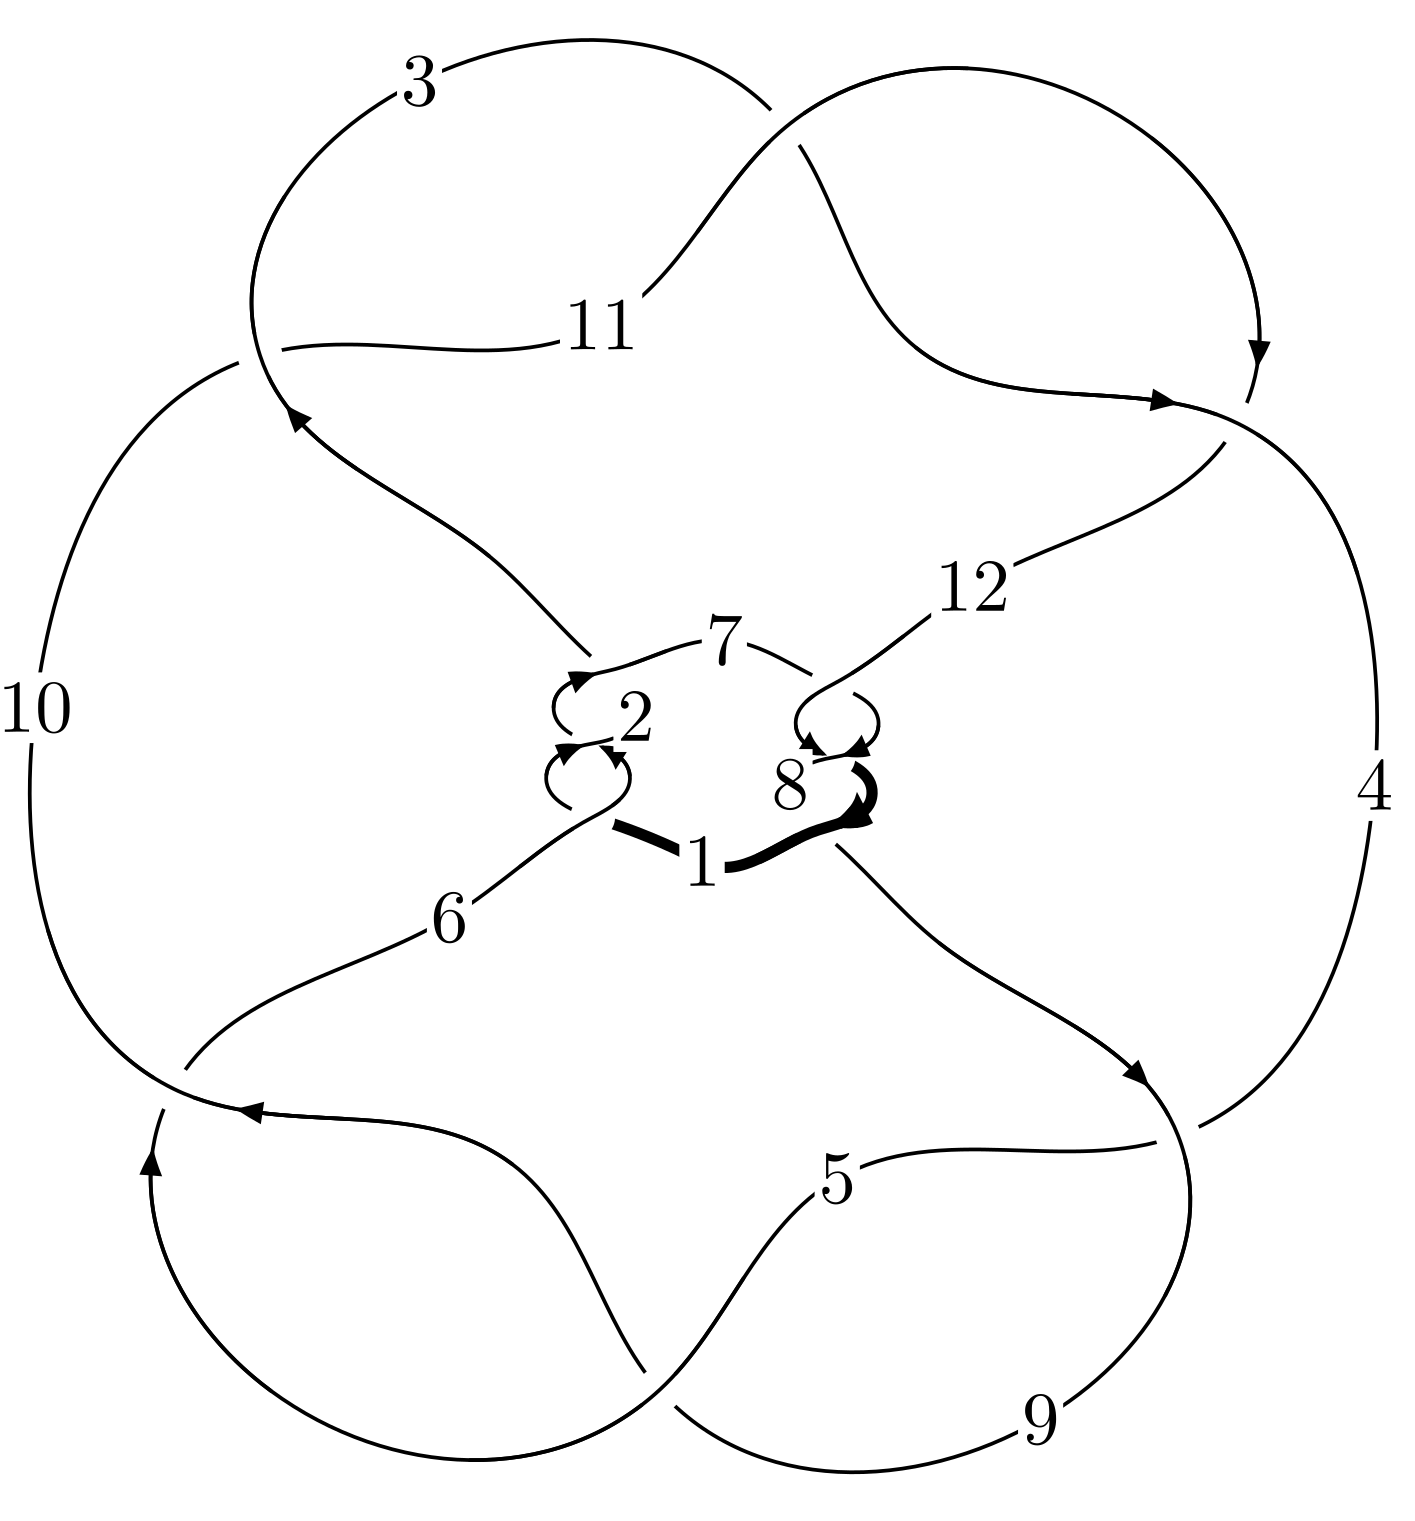
\includegraphics[width=112pt]{../../../GIT/diagram.site/Diagrams/png/2089_12a_1288.png}\\
\ \ \ A knot diagram\footnotemark}&
\allowdisplaybreaks
\textbf{Linearized knot diagam} \\
\cline{2-2}
 &
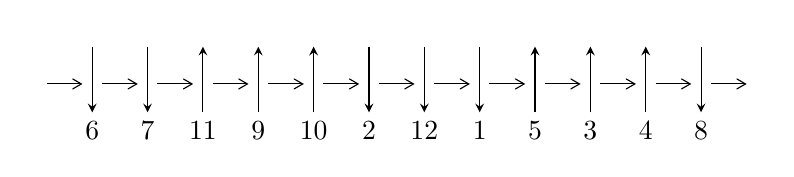
\begin{tikzpicture}[x=20pt, y=17pt]
	% nodes
	\node (C0) at (0, 0) {};
	\node (C1) at (1, 0) {};
	\node (C1U) at (1, +1) {};
	\node (C1D) at (1, -1) {6};

	\node (C2) at (2, 0) {};
	\node (C2U) at (2, +1) {};
	\node (C2D) at (2, -1) {7};

	\node (C3) at (3, 0) {};
	\node (C3U) at (3, +1) {};
	\node (C3D) at (3, -1) {11};

	\node (C4) at (4, 0) {};
	\node (C4U) at (4, +1) {};
	\node (C4D) at (4, -1) {9};

	\node (C5) at (5, 0) {};
	\node (C5U) at (5, +1) {};
	\node (C5D) at (5, -1) {10};

	\node (C6) at (6, 0) {};
	\node (C6U) at (6, +1) {};
	\node (C6D) at (6, -1) {2};

	\node (C7) at (7, 0) {};
	\node (C7U) at (7, +1) {};
	\node (C7D) at (7, -1) {12};

	\node (C8) at (8, 0) {};
	\node (C8U) at (8, +1) {};
	\node (C8D) at (8, -1) {1};

	\node (C9) at (9, 0) {};
	\node (C9U) at (9, +1) {};
	\node (C9D) at (9, -1) {5};

	\node (C10) at (10, 0) {};
	\node (C10U) at (10, +1) {};
	\node (C10D) at (10, -1) {3};

	\node (C11) at (11, 0) {};
	\node (C11U) at (11, +1) {};
	\node (C11D) at (11, -1) {4};

	\node (C12) at (12, 0) {};
	\node (C12U) at (12, +1) {};
	\node (C12D) at (12, -1) {8};
	\node (C13) at (13, 0) {};

	% arrows
	\draw[->,>={angle 60}]
	(C0) edge (C1) (C1) edge (C2) (C2) edge (C3) (C3) edge (C4) (C4) edge (C5) (C5) edge (C6) (C6) edge (C7) (C7) edge (C8) (C8) edge (C9) (C9) edge (C10) (C10) edge (C11) (C11) edge (C12) (C12) edge (C13) ;	\draw[->,>=stealth]
	(C1U) edge (C1D) (C2U) edge (C2D) (C3D) edge (C3U) (C4D) edge (C4U) (C5D) edge (C5U) (C6U) edge (C6D) (C7U) edge (C7D) (C8U) edge (C8D) (C9D) edge (C9U) (C10D) edge (C10U) (C11D) edge (C11U) (C12U) edge (C12D) ;
	\end{tikzpicture} \\
\hhline{~~} \\& 
\textbf{Solving Sequence} \\ \cline{2-2} 
 &
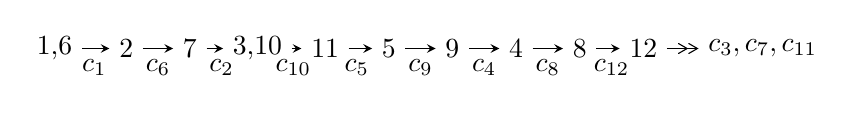
\begin{tikzpicture}[x=23pt, y=7pt]
	% node
	\node (A0) at (-1/8, 0) {1,6};
	\node (A1) at (1, 0) {2};
	\node (A2) at (2, 0) {7};
	\node (A3) at (49/16, 0) {3,10};
	\node (A4) at (33/8, 0) {11};
	\node (A5) at (41/8, 0) {5};
	\node (A6) at (49/8, 0) {9};
	\node (A7) at (57/8, 0) {4};
	\node (A8) at (65/8, 0) {8};
	\node (A9) at (73/8, 0) {12};
	\node (C1) at (1/2, -1) {$c_{1}$};
	\node (C2) at (3/2, -1) {$c_{6}$};
	\node (C3) at (5/2, -1) {$c_{2}$};
	\node (C4) at (29/8, -1) {$c_{10}$};
	\node (C5) at (37/8, -1) {$c_{5}$};
	\node (C6) at (45/8, -1) {$c_{9}$};
	\node (C7) at (53/8, -1) {$c_{4}$};
	\node (C8) at (61/8, -1) {$c_{8}$};
	\node (C9) at (69/8, -1) {$c_{12}$};
	\node (A10) at (11, 0) {$c_{3},c_{7},c_{11}$};

	% edge
	\draw[->,>=stealth]	
	(A0) edge (A1) (A1) edge (A2) (A2) edge (A3) (A3) edge (A4) (A4) edge (A5) (A5) edge (A6) (A6) edge (A7) (A7) edge (A8) (A8) edge (A9) ;
	\draw[->>,>={angle 60}]	
	(A9) edge (A10);
\end{tikzpicture} \\ 

\end{tabular} \\

\footnotetext{
The image of knot diagram is generated by the software ``\textbf{Draw programme}" developed by Andrew Bartholomew(\url{http://www.layer8.co.uk/maths/draw/index.htm\#Running-draw}), where we modified some parts for our purpose(\url{https://github.com/CATsTAILs/LinksPainter}).
}\phantom \\ \newline 
\centering \textbf{Ideals for irreducible components\footnotemark of $X_{\text{par}}$} 
 
\begin{align*}
I^u_{1}&=\langle 
u^{11}+u^{10}-6 u^9-5 u^8+11 u^7+5 u^6-7 u^5+5 u^4+3 u^3-4 u^2+4 b-2 u,\\
\phantom{I^u_{1}}&\phantom{= \langle  }-3 u^{11}-8 u^{10}+9 u^9+33 u^8-4 u^7-30 u^6+20 u^5-42 u^3+u^2+4 a+10 u-2,\\
\phantom{I^u_{1}}&\phantom{= \langle  }u^{12}+3 u^{11}-3 u^{10}-14 u^9+u^8+18 u^7-8 u^6-6 u^5+24 u^4-3 u^3-13 u^2+6 u-2\rangle \\
I^u_{2}&=\langle 
1999 u^{15}+3106 u^{14}+\cdots+2878 b-22827,\;-1627 u^{15}-1680 u^{14}+\cdots+15829 a+36947,\\
\phantom{I^u_{2}}&\phantom{= \langle  }u^{16}+3 u^{15}+\cdots-2 u-11\rangle \\
I^u_{3}&=\langle 
u^7 a- u^7-4 u^5 a- u^4 a+4 u^5+4 u^3 a- u^4+u^2 a-4 u^3+2 a u+u^2+2 b+a+1,\\
\phantom{I^u_{3}}&\phantom{= \langle  }- u^7 a+u^6 a+2 u^7+3 u^5 a-3 u^6-3 u^4 a-7 u^5-2 u^3 a+10 u^4+2 u^2 a+7 u^3+a^2- a u-7 u^2+a-5,\\
\phantom{I^u_{3}}&\phantom{= \langle  }u^8- u^7-4 u^6+3 u^5+5 u^4- u^3- u^2-3 u-1\rangle \\
I^u_{4}&=\langle 
- u^{11} a- u^{11}+\cdots+a+1,\\
\phantom{I^u_{4}}&\phantom{= \langle  }u^{11}-5 u^9+u^7 a-2 u^8+9 u^7-2 u^5 a+8 u^6- u^4 a-4 u^5-10 u^4+u^2 a-6 u^3+a^2+2 a u+2 u^2+a+6 u+2,\\
\phantom{I^u_{4}}&\phantom{= \langle  }u^{12}- u^{11}-4 u^{10}+2 u^9+7 u^8+u^7-5 u^6-5 u^5- u^4+3 u^3+2 u^2+1\rangle \\
I^u_{5}&=\langle 
2 b- a-1,\;a^2-3,\;u-1\rangle \\
I^u_{6}&=\langle 
2 b- u+1,\;3 a- u,\;u^2-3\rangle \\
I^u_{7}&=\langle 
b+1,\;a,\;u-1\rangle \\
I^u_{8}&=\langle 
4 b^2-4 b+5,\;2 b a-2 b-3 a+4 u+7,\;2 b u+2 b-2 a+u+3,\;a^2-2 a+1,\;a u+a- u-1,\;u^2+2 u+1\rangle \\
I^u_{9}&=\langle 
a-1,\;u+1\rangle \\
\\
I^v_{1}&=\langle 
a,\;b-1,\;v+1\rangle \\
\end{align*}
\raggedright * 9 irreducible components of $\dim_{\mathbb{C}}=0$, with total 78 representations.\\
\raggedright * 1 irreducible components of $\dim_{\mathbb{C}}=1$ \\
\footnotetext{All coefficients of polynomials are rational numbers. But the coefficients are sometimes approximated in decimal forms when there is not enough margin.}
\newpage
\renewcommand{\arraystretch}{1}
\centering \section*{I. $I^u_{1}= \langle u^{11}+u^{10}+\cdots+4 b-2 u,\;-3 u^{11}-8 u^{10}+\cdots+4 a-2,\;u^{12}+3 u^{11}+\cdots+6 u-2 \rangle$}
\flushleft \textbf{(i) Arc colorings}\\
\begin{tabular}{m{7pt} m{180pt} m{7pt} m{180pt} }
\flushright $a_{1}=$&$\begin{pmatrix}1\\0\end{pmatrix}$ \\
\flushright $a_{6}=$&$\begin{pmatrix}0\\u\end{pmatrix}$ \\
\flushright $a_{2}=$&$\begin{pmatrix}1\\u^2\end{pmatrix}$ \\
\flushright $a_{7}=$&$\begin{pmatrix}- u\\- u^3+u\end{pmatrix}$ \\
\flushright $a_{3}=$&$\begin{pmatrix}- u^2+1\\- u^4+2 u^2\end{pmatrix}$ \\
\flushright $a_{10}=$&$\begin{pmatrix}\frac{3}{4} u^{11}+2 u^{10}+\cdots-\frac{5}{2} u+\frac{1}{2}\\-\frac{1}{4} u^{11}-\frac{1}{4} u^{10}+\cdots+u^2+\frac{1}{2} u\end{pmatrix}$ \\
\flushright $a_{11}=$&$\begin{pmatrix}\frac{1}{4} u^{11}+u^{10}+\cdots-\frac{7}{2} u+\frac{1}{2}\\-\frac{1}{4} u^{10}-\frac{3}{4} u^9+\cdots+\frac{3}{2} u-\frac{1}{2}\end{pmatrix}$ \\
\flushright $a_{5}=$&$\begin{pmatrix}-\frac{1}{4} u^{11}- u^{10}+\cdots+\frac{3}{2} u-\frac{1}{2}\\-\frac{1}{4} u^{11}-\frac{1}{4} u^{10}+\cdots+u^2+\frac{1}{2} u\end{pmatrix}$ \\
\flushright $a_{9}=$&$\begin{pmatrix}-\frac{1}{2} u^{10}-\frac{3}{2} u^9+\cdots-\frac{15}{2} u^2-1\\u\end{pmatrix}$ \\
\flushright $a_{4}=$&$\begin{pmatrix}-\frac{1}{4} u^{11}+\frac{7}{4} u^9+\cdots-\frac{3}{2} u+\frac{3}{2}\\- u^{11}-\frac{7}{4} u^{10}+\cdots-\frac{5}{2} u+\frac{1}{2}\end{pmatrix}$ \\
\flushright $a_{8}=$&$\begin{pmatrix}-\frac{1}{2} u^{10}-\frac{3}{2} u^9+\cdots+u-1\\u\end{pmatrix}$ \\
\flushright $a_{12}=$&$\begin{pmatrix}\frac{1}{2} u^{11}+\frac{3}{2} u^{10}+\cdots+u+1\\- u^2\end{pmatrix}$\\&\end{tabular}
\flushleft \textbf{(ii) Obstruction class $= -1$}\\~\\
\flushleft \textbf{(iii) Cusp Shapes $= \frac{1}{2} u^{11}+u^{10}-\frac{3}{2} u^9-\frac{1}{2} u^8+3 u^7-13 u^6-8 u^5+22 u^4-11 u^3-\frac{19}{2} u^2+32 u-7$}\\~\\
\newpage\renewcommand{\arraystretch}{1}
\flushleft \textbf{(iv) u-Polynomials at the component}\newline \\
\begin{tabular}{m{50pt}|m{274pt}}
Crossings & \hspace{64pt}u-Polynomials at each crossing \\
\hline $$\begin{aligned}c_{1},c_{2},c_{6}\\c_{7},c_{8},c_{12}\end{aligned}$$&$\begin{aligned}
&u^{12}-3 u^{11}+\cdots-6 u-2
\end{aligned}$\\
\hline $$\begin{aligned}c_{3},c_{4},c_{5}\\c_{9},c_{10},c_{11}\end{aligned}$$&$\begin{aligned}
&u^{12}+3 u^{11}+\cdots+6 u-2
\end{aligned}$\\
\hline
\end{tabular}\\~\\
\newpage\renewcommand{\arraystretch}{1}
\flushleft \textbf{(v) Riley Polynomials at the component}\newline \\
\begin{tabular}{m{50pt}|m{274pt}}
Crossings & \hspace{64pt}Riley Polynomials at each crossing \\
\hline $$\begin{aligned}c_{1},c_{2},c_{3}\\c_{4},c_{5},c_{6}\\c_{7},c_{8},c_{9}\\c_{10},c_{11},c_{12}\end{aligned}$$&$\begin{aligned}
&y^{12}-15 y^{11}+\cdots+16 y+4
\end{aligned}$\\
\hline
\end{tabular}\\~\\
\newpage\flushleft \textbf{(vi) Complex Volumes and Cusp Shapes}
$$\begin{array}{c|c|c}  
\text{Solutions to }I^u_{1}& \I (\text{vol} + \sqrt{-1}CS) & \text{Cusp shape}\\
 \hline 
\begin{aligned}
u &= \phantom{-}0.369891 + 0.895594 I \\
a &= -0.40167 + 1.49298 I \\
b &= -0.02653 - 1.85453 I\end{aligned}
 & \phantom{-}11.33630 - 5.25212 I & \phantom{-}7.30257 + 4.65184 I \\ \hline\begin{aligned}
u &= \phantom{-}0.369891 - 0.895594 I \\
a &= -0.40167 - 1.49298 I \\
b &= -0.02653 + 1.85453 I\end{aligned}
 & \phantom{-}11.33630 + 5.25212 I & \phantom{-}7.30257 - 4.65184 I \\ \hline\begin{aligned}
u &= \phantom{-}1.22438\phantom{ +0.000000I} \\
a &= -1.51331\phantom{ +0.000000I} \\
b &= -1.43561\phantom{ +0.000000I}\end{aligned}
 & \phantom{-}8.64658\phantom{ +0.000000I} & -5.83920\phantom{ +0.000000I} \\ \hline\begin{aligned}
u &= \phantom{-}0.740748\phantom{ +0.000000I} \\
a &= \phantom{-}2.25319\phantom{ +0.000000I} \\
b &= \phantom{-}0.277533\phantom{ +0.000000I}\end{aligned}
 & \phantom{-}10.7798\phantom{ +0.000000I} & \phantom{-}10.0010\phantom{ +0.000000I} \\ \hline\begin{aligned}
u &= -1.48568 + 0.19251 I \\
a &= -0.168040 - 0.624592 I \\
b &= -0.695418 + 0.595170 I\end{aligned}
 & -11.33630 + 5.25212 I & -7.30257 - 4.65184 I \\ \hline\begin{aligned}
u &= -1.48568 - 0.19251 I \\
a &= -0.168040 + 0.624592 I \\
b &= -0.695418 - 0.595170 I\end{aligned}
 & -11.33630 - 5.25212 I & -7.30257 + 4.65184 I \\ \hline\begin{aligned}
u &= -1.46094 + 0.44342 I \\
a &= \phantom{-}0.831296 + 0.555829 I \\
b &= \phantom{-}1.16548 - 2.08317 I\end{aligned}
 & \phantom{-0.000000 -}15.2352 I & \phantom{-0.000000 } 0. - 7.62682 I \\ \hline\begin{aligned}
u &= -1.46094 - 0.44342 I \\
a &= \phantom{-}0.831296 - 0.555829 I \\
b &= \phantom{-}1.16548 + 2.08317 I\end{aligned}
 & \phantom{-0.000000 } -15.2352 I & \phantom{-0.000000 -}0. + 7.62682 I \\ \hline\begin{aligned}
u &= \phantom{-}0.186071 + 0.332496 I \\
a &= -0.523030 - 0.852314 I \\
b &= \phantom{-}0.072588 + 0.300683 I\end{aligned}
 & \phantom{-0.000000 } -0.761015 I & \phantom{-0.000000 -}0. + 9.12858 I \\ \hline\begin{aligned}
u &= \phantom{-}0.186071 - 0.332496 I \\
a &= -0.523030 + 0.852314 I \\
b &= \phantom{-}0.072588 - 0.300683 I\end{aligned}
 & \phantom{-0.000000 -}0.761015 I & \phantom{-0.000000 } 0. - 9.12858 I\\
 \hline 
 \end{array}$$\newpage$$\begin{array}{c|c|c}  
\text{Solutions to }I^u_{1}& \I (\text{vol} + \sqrt{-1}CS) & \text{Cusp shape}\\
 \hline 
\begin{aligned}
u &= \phantom{-}1.66904\phantom{ +0.000000I} \\
a &= \phantom{-}0.443816\phantom{ +0.000000I} \\
b &= \phantom{-}0.958809\phantom{ +0.000000I}\end{aligned}
 & -10.7798\phantom{ +0.000000I} & -10.0010\phantom{ +0.000000I} \\ \hline\begin{aligned}
u &= -1.85286\phantom{ +0.000000I} \\
a &= -0.660804\phantom{ +0.000000I} \\
b &= -0.832979\phantom{ +0.000000I}\end{aligned}
 & -8.64658\phantom{ +0.000000I} & \phantom{-}5.83920\phantom{ +0.000000I}\\
 \hline 
 \end{array}$$\newpage\newpage\renewcommand{\arraystretch}{1}
\centering \section*{II. $I^u_{2}= \langle 1999 u^{15}+3106 u^{14}+\cdots+2878 b-22827,\;-1627 u^{15}-1680 u^{14}+\cdots+15829 a+36947,\;u^{16}+3 u^{15}+\cdots-2 u-11 \rangle$}
\flushleft \textbf{(i) Arc colorings}\\
\begin{tabular}{m{7pt} m{180pt} m{7pt} m{180pt} }
\flushright $a_{1}=$&$\begin{pmatrix}1\\0\end{pmatrix}$ \\
\flushright $a_{6}=$&$\begin{pmatrix}0\\u\end{pmatrix}$ \\
\flushright $a_{2}=$&$\begin{pmatrix}1\\u^2\end{pmatrix}$ \\
\flushright $a_{7}=$&$\begin{pmatrix}- u\\- u^3+u\end{pmatrix}$ \\
\flushright $a_{3}=$&$\begin{pmatrix}- u^2+1\\- u^4+2 u^2\end{pmatrix}$ \\
\flushright $a_{10}=$&$\begin{pmatrix}0.102786 u^{15}+0.106134 u^{14}+\cdots-0.0633647 u-2.33413\\-0.694580 u^{15}-1.07922 u^{14}+\cdots-5.24913 u+7.93155\end{pmatrix}$ \\
\flushright $a_{11}=$&$\begin{pmatrix}0.0812433 u^{15}+0.190220 u^{14}+\cdots+0.503696 u+0.181502\\-1.01355 u^{15}-1.80195 u^{14}+\cdots-3.62717 u+5.92113\end{pmatrix}$ \\
\flushright $a_{5}=$&$\begin{pmatrix}0.0504138 u^{15}-0.0794744 u^{14}+\cdots+1.94864 u+1.81092\\0.312370 u^{15}+0.280751 u^{14}+\cdots+1.27762 u-4.97672\end{pmatrix}$ \\
\flushright $a_{9}=$&$\begin{pmatrix}0.503254 u^{15}+0.504896 u^{14}+\cdots+3.85571 u-3.97524\\-0.594163 u^{15}-0.777623 u^{14}+\cdots-6.03753 u+4.15705\end{pmatrix}$ \\
\flushright $a_{4}=$&$\begin{pmatrix}0.434645 u^{15}+0.605534 u^{14}+\cdots+2.21884 u-1.80814\\0.0309243 u^{15}-0.298124 u^{14}+\cdots+0.944058 u-3.69180\end{pmatrix}$ \\
\flushright $a_{8}=$&$\begin{pmatrix}-0.0909091 u^{15}-0.272727 u^{14}+\cdots-2.18182 u+0.181818\\-0.594163 u^{15}-0.777623 u^{14}+\cdots-6.03753 u+4.15705\end{pmatrix}$ \\
\flushright $a_{12}=$&$\begin{pmatrix}0.377914 u^{15}+0.539579 u^{14}+\cdots+1.33679 u-5.79335\\1.00486 u^{15}+1.85198 u^{14}+\cdots+2.96873 u-7.53579\end{pmatrix}$\\&\end{tabular}
\flushleft \textbf{(ii) Obstruction class $= -1$}\\~\\
\flushleft \textbf{(iii) Cusp Shapes $= -\frac{3610}{1439} u^{15}-\frac{5684}{1439} u^{14}+\cdots-\frac{43398}{1439} u+\frac{24298}{1439}$}\\~\\
\newpage\renewcommand{\arraystretch}{1}
\flushleft \textbf{(iv) u-Polynomials at the component}\newline \\
\begin{tabular}{m{50pt}|m{274pt}}
Crossings & \hspace{64pt}u-Polynomials at each crossing \\
\hline $$\begin{aligned}c_{1},c_{2},c_{6}\\c_{7},c_{8},c_{12}\end{aligned}$$&$\begin{aligned}
&u^{16}-3 u^{15}+\cdots+2 u-11
\end{aligned}$\\
\hline $$\begin{aligned}c_{3},c_{4},c_{5}\\c_{9},c_{10},c_{11}\end{aligned}$$&$\begin{aligned}
&(u^8- u^7-4 u^6+3 u^5+5 u^4- u^3- u^2-3 u-1)^2
\end{aligned}$\\
\hline
\end{tabular}\\~\\
\newpage\renewcommand{\arraystretch}{1}
\flushleft \textbf{(v) Riley Polynomials at the component}\newline \\
\begin{tabular}{m{50pt}|m{274pt}}
Crossings & \hspace{64pt}Riley Polynomials at each crossing \\
\hline $$\begin{aligned}c_{1},c_{2},c_{6}\\c_{7},c_{8},c_{12}\end{aligned}$$&$\begin{aligned}
&y^{16}-13 y^{15}+\cdots-532 y+121
\end{aligned}$\\
\hline $$\begin{aligned}c_{3},c_{4},c_{5}\\c_{9},c_{10},c_{11}\end{aligned}$$&$\begin{aligned}
&(y^8-9 y^7+32 y^6-53 y^5+31 y^4+15 y^3-15 y^2-7 y+1)^2
\end{aligned}$\\
\hline
\end{tabular}\\~\\
\newpage\flushleft \textbf{(vi) Complex Volumes and Cusp Shapes}
$$\begin{array}{c|c|c}  
\text{Solutions to }I^u_{2}& \I (\text{vol} + \sqrt{-1}CS) & \text{Cusp shape}\\
 \hline 
\begin{aligned}
u &= \phantom{-}0.694226 + 0.667719 I \\
a &= \phantom{-}1.12920 - 1.08608 I \\
b &= \phantom{-}0.276681 + 1.311520 I\end{aligned}
 & \phantom{-}10.1546\phantom{ +0.000000I} & \phantom{-}6.33746 + 0. I\phantom{ +0.000000I} \\ \hline\begin{aligned}
u &= \phantom{-}0.694226 - 0.667719 I \\
a &= \phantom{-}1.12920 + 1.08608 I \\
b &= \phantom{-}0.276681 - 1.311520 I\end{aligned}
 & \phantom{-}10.1546\phantom{ +0.000000I} & \phantom{-}6.33746 + 0. I\phantom{ +0.000000I} \\ \hline\begin{aligned}
u &= \phantom{-}0.262333 + 1.058630 I \\
a &= \phantom{-}0.019128 - 1.343770 I \\
b &= \phantom{-}0.19190 + 2.13545 I\end{aligned}
 & \phantom{-}5.44991 - 9.88301 I & \phantom{-}3.28252 + 6.06963 I \\ \hline\begin{aligned}
u &= \phantom{-}0.262333 - 1.058630 I \\
a &= \phantom{-}0.019128 + 1.343770 I \\
b &= \phantom{-}0.19190 - 2.13545 I\end{aligned}
 & \phantom{-}5.44991 + 9.88301 I & \phantom{-}3.28252 - 6.06963 I \\ \hline\begin{aligned}
u &= \phantom{-}1.15427\phantom{ +0.000000I} \\
a &= -0.296909\phantom{ +0.000000I} \\
b &= -0.236501\phantom{ +0.000000I}\end{aligned}
 & -2.57083\phantom{ +0.000000I} & \phantom{-}2.16010\phantom{ +0.000000I} \\ \hline\begin{aligned}
u &= \phantom{-}0.524313 + 0.657146 I \\
a &= \phantom{-}0.513557 + 0.640043 I \\
b &= -0.598451 - 0.154997 I\end{aligned}
 & -4.77492 - 2.26376 I & -6.05872 + 4.53378 I \\ \hline\begin{aligned}
u &= \phantom{-}0.524313 - 0.657146 I \\
a &= \phantom{-}0.513557 - 0.640043 I \\
b &= -0.598451 + 0.154997 I\end{aligned}
 & -4.77492 + 2.26376 I & -6.05872 - 4.53378 I \\ \hline\begin{aligned}
u &= -1.345930 + 0.090134 I \\
a &= \phantom{-}0.078599 + 0.505339 I \\
b &= \phantom{-}0.329421 - 1.036490 I\end{aligned}
 & -4.77492 + 2.26376 I & -6.05872 - 4.53378 I \\ \hline\begin{aligned}
u &= -1.345930 - 0.090134 I \\
a &= \phantom{-}0.078599 - 0.505339 I \\
b &= \phantom{-}0.329421 + 1.036490 I\end{aligned}
 & -4.77492 - 2.26376 I & -6.05872 + 4.53378 I \\ \hline\begin{aligned}
u &= \phantom{-}1.125920 + 0.800303 I \\
a &= -0.889080 + 0.447838 I \\
b &= -0.77247 - 1.44681 I\end{aligned}
 & \phantom{-}2.93531 + 3.55755 I & \phantom{-}2.52739 - 2.62489 I\\
 \hline 
 \end{array}$$\newpage$$\begin{array}{c|c|c}  
\text{Solutions to }I^u_{2}& \I (\text{vol} + \sqrt{-1}CS) & \text{Cusp shape}\\
 \hline 
\begin{aligned}
u &= \phantom{-}1.125920 - 0.800303 I \\
a &= -0.889080 - 0.447838 I \\
b &= -0.77247 + 1.44681 I\end{aligned}
 & \phantom{-}2.93531 - 3.55755 I & \phantom{-}2.52739 + 2.62489 I \\ \hline\begin{aligned}
u &= -0.604309\phantom{ +0.000000I} \\
a &= \phantom{-}0.567118\phantom{ +0.000000I} \\
b &= \phantom{-}1.07322\phantom{ +0.000000I}\end{aligned}
 & -2.57083\phantom{ +0.000000I} & \phantom{-}2.16010\phantom{ +0.000000I} \\ \hline\begin{aligned}
u &= -1.47759 + 0.37462 I \\
a &= -0.854231 - 0.441448 I \\
b &= -0.72115 + 1.92612 I\end{aligned}
 & \phantom{-}5.44991 + 9.88301 I & \phantom{-}3.28252 - 6.06963 I \\ \hline\begin{aligned}
u &= -1.47759 - 0.37462 I \\
a &= -0.854231 + 0.441448 I \\
b &= -0.72115 - 1.92612 I\end{aligned}
 & \phantom{-}5.44991 - 9.88301 I & \phantom{-}3.28252 + 6.06963 I \\ \hline\begin{aligned}
u &= -1.55826 + 0.27885 I \\
a &= \phantom{-}0.822270 + 0.280177 I \\
b &= \phantom{-}0.375716 - 1.326680 I\end{aligned}
 & \phantom{-}2.93531 + 3.55755 I & \phantom{-}2.52739 - 2.62489 I \\ \hline\begin{aligned}
u &= -1.55826 - 0.27885 I \\
a &= \phantom{-}0.822270 - 0.280177 I \\
b &= \phantom{-}0.375716 + 1.326680 I\end{aligned}
 & \phantom{-}2.93531 - 3.55755 I & \phantom{-}2.52739 + 2.62489 I\\
 \hline 
 \end{array}$$\newpage\newpage\renewcommand{\arraystretch}{1}
\centering \section*{III. $I^u_{3}= \langle u^7 a- u^7+\cdots+a+1,\;- u^7 a+2 u^7+\cdots+a-5,\;u^8- u^7-4 u^6+3 u^5+5 u^4- u^3- u^2-3 u-1 \rangle$}
\flushleft \textbf{(i) Arc colorings}\\
\begin{tabular}{m{7pt} m{180pt} m{7pt} m{180pt} }
\flushright $a_{1}=$&$\begin{pmatrix}1\\0\end{pmatrix}$ \\
\flushright $a_{6}=$&$\begin{pmatrix}0\\u\end{pmatrix}$ \\
\flushright $a_{2}=$&$\begin{pmatrix}1\\u^2\end{pmatrix}$ \\
\flushright $a_{7}=$&$\begin{pmatrix}- u\\- u^3+u\end{pmatrix}$ \\
\flushright $a_{3}=$&$\begin{pmatrix}- u^2+1\\- u^4+2 u^2\end{pmatrix}$ \\
\flushright $a_{10}=$&$\begin{pmatrix}a\\-\frac{1}{2} u^7 a+\frac{1}{2} u^7+\cdots-\frac{1}{2} a-\frac{1}{2}\end{pmatrix}$ \\
\flushright $a_{11}=$&$\begin{pmatrix}u^7-4 u^5- u^3 a+4 u^3+a u+a+u\\-\frac{1}{2} u^7 a+\frac{1}{2} u^7+\cdots-\frac{1}{2} a-\frac{1}{2}\end{pmatrix}$ \\
\flushright $a_{5}=$&$\begin{pmatrix}- u^6 a- u^7+\cdots- a+2\\-\frac{1}{2} u^7 a+\frac{1}{2} u^7+\cdots-\frac{1}{2} a-\frac{1}{2}\end{pmatrix}$ \\
\flushright $a_{9}=$&$\begin{pmatrix}u^6- u^5-3 u^4+2 u^3+2 u^2+1\\u\end{pmatrix}$ \\
\flushright $a_{4}=$&$\begin{pmatrix}- u^7 a- u^7+\cdots- a+2\\-\frac{1}{2} u^7 a+\frac{1}{2} u^7+\cdots-\frac{1}{2} a-\frac{1}{2}\end{pmatrix}$ \\
\flushright $a_{8}=$&$\begin{pmatrix}u^6- u^5-3 u^4+2 u^3+2 u^2+u+1\\u\end{pmatrix}$ \\
\flushright $a_{12}=$&$\begin{pmatrix}- u^7+u^6+3 u^5-2 u^4-2 u^3- u^2- u+1\\- u^2\end{pmatrix}$\\&\end{tabular}
\flushleft \textbf{(ii) Obstruction class $= -1$}\\~\\
\flushleft \textbf{(iii) Cusp Shapes $= -2 u^6-2 u^5+10 u^4+8 u^3-12 u^2-10 u-4$}\\~\\
\newpage\renewcommand{\arraystretch}{1}
\flushleft \textbf{(iv) u-Polynomials at the component}\newline \\
\begin{tabular}{m{50pt}|m{274pt}}
Crossings & \hspace{64pt}u-Polynomials at each crossing \\
\hline $$\begin{aligned}c_{1},c_{2},c_{6}\\c_{7},c_{8},c_{12}\end{aligned}$$&$\begin{aligned}
&(u^8+u^7-4 u^6-3 u^5+5 u^4+u^3- u^2+3 u-1)^2
\end{aligned}$\\
\hline $$\begin{aligned}c_{3},c_{4},c_{5}\\c_{9},c_{10},c_{11}\end{aligned}$$&$\begin{aligned}
&u^{16}+3 u^{15}+\cdots-2 u-11
\end{aligned}$\\
\hline
\end{tabular}\\~\\
\newpage\renewcommand{\arraystretch}{1}
\flushleft \textbf{(v) Riley Polynomials at the component}\newline \\
\begin{tabular}{m{50pt}|m{274pt}}
Crossings & \hspace{64pt}Riley Polynomials at each crossing \\
\hline $$\begin{aligned}c_{1},c_{2},c_{6}\\c_{7},c_{8},c_{12}\end{aligned}$$&$\begin{aligned}
&(y^8-9 y^7+32 y^6-53 y^5+31 y^4+15 y^3-15 y^2-7 y+1)^2
\end{aligned}$\\
\hline $$\begin{aligned}c_{3},c_{4},c_{5}\\c_{9},c_{10},c_{11}\end{aligned}$$&$\begin{aligned}
&y^{16}-13 y^{15}+\cdots-532 y+121
\end{aligned}$\\
\hline
\end{tabular}\\~\\
\newpage\flushleft \textbf{(vi) Complex Volumes and Cusp Shapes}
$$\begin{array}{c|c|c}  
\text{Solutions to }I^u_{3}& \I (\text{vol} + \sqrt{-1}CS) & \text{Cusp shape}\\
 \hline 
\begin{aligned}
u &= -0.151337 + 0.673064 I \\
a &= \phantom{-}0.762637 - 0.950471 I \\
b &= \phantom{-}0.076801 + 0.408443 I\end{aligned}
 & \phantom{-}4.77492 + 2.26376 I & \phantom{-}6.05872 - 4.53378 I \\ \hline\begin{aligned}
u &= -0.151337 + 0.673064 I \\
a &= \phantom{-}0.30052 + 1.93213 I \\
b &= -0.06507 - 1.92874 I\end{aligned}
 & \phantom{-}4.77492 + 2.26376 I & \phantom{-}6.05872 - 4.53378 I \\ \hline\begin{aligned}
u &= -0.151337 - 0.673064 I \\
a &= \phantom{-}0.762637 + 0.950471 I \\
b &= \phantom{-}0.076801 - 0.408443 I\end{aligned}
 & \phantom{-}4.77492 - 2.26376 I & \phantom{-}6.05872 + 4.53378 I \\ \hline\begin{aligned}
u &= -0.151337 - 0.673064 I \\
a &= \phantom{-}0.30052 - 1.93213 I \\
b &= -0.06507 + 1.92874 I\end{aligned}
 & \phantom{-}4.77492 - 2.26376 I & \phantom{-}6.05872 + 4.53378 I \\ \hline\begin{aligned}
u &= -1.359440 + 0.207304 I \\
a &= -0.897134 + 0.451895 I \\
b &= -0.592239 - 0.125436 I\end{aligned}
 & -2.93531 + 3.55755 I & -2.52739 - 2.62489 I \\ \hline\begin{aligned}
u &= -1.359440 + 0.207304 I \\
a &= \phantom{-}1.089640 + 0.371279 I \\
b &= \phantom{-}1.80045 - 1.27064 I\end{aligned}
 & -2.93531 + 3.55755 I & -2.52739 - 2.62489 I \\ \hline\begin{aligned}
u &= -1.359440 - 0.207304 I \\
a &= -0.897134 - 0.451895 I \\
b &= -0.592239 + 0.125436 I\end{aligned}
 & -2.93531 - 3.55755 I & -2.52739 + 2.62489 I \\ \hline\begin{aligned}
u &= -1.359440 - 0.207304 I \\
a &= \phantom{-}1.089640 - 0.371279 I \\
b &= \phantom{-}1.80045 + 1.27064 I\end{aligned}
 & -2.93531 - 3.55755 I & -2.52739 + 2.62489 I \\ \hline\begin{aligned}
u &= \phantom{-}1.42757 + 0.33227 I \\
a &= -0.923905 + 0.477454 I \\
b &= -1.51269 - 1.88228 I\end{aligned}
 & -5.44991 - 9.88301 I & -3.28252 + 6.06963 I \\ \hline\begin{aligned}
u &= \phantom{-}1.42757 + 0.33227 I \\
a &= \phantom{-}0.010591 - 0.744025 I \\
b &= \phantom{-}0.534351 + 0.711339 I\end{aligned}
 & -5.44991 - 9.88301 I & -3.28252 + 6.06963 I\\
 \hline 
 \end{array}$$\newpage$$\begin{array}{c|c|c}  
\text{Solutions to }I^u_{3}& \I (\text{vol} + \sqrt{-1}CS) & \text{Cusp shape}\\
 \hline 
\begin{aligned}
u &= \phantom{-}1.42757 - 0.33227 I \\
a &= -0.923905 - 0.477454 I \\
b &= -1.51269 + 1.88228 I\end{aligned}
 & -5.44991 + 9.88301 I & -3.28252 - 6.06963 I \\ \hline\begin{aligned}
u &= \phantom{-}1.42757 - 0.33227 I \\
a &= \phantom{-}0.010591 + 0.744025 I \\
b &= \phantom{-}0.534351 - 0.711339 I\end{aligned}
 & -5.44991 + 9.88301 I & -3.28252 - 6.06963 I \\ \hline\begin{aligned}
u &= \phantom{-}1.50912\phantom{ +0.000000I} \\
a &= \phantom{-}0.460021 + 0.442457 I \\
b &= \phantom{-}0.770987 - 0.303857 I\end{aligned}
 & -10.1546\phantom{ +0.000000I} & -6.33750\phantom{ +0.000000I} \\ \hline\begin{aligned}
u &= \phantom{-}1.50912\phantom{ +0.000000I} \\
a &= \phantom{-}0.460021 - 0.442457 I \\
b &= \phantom{-}0.770987 + 0.303857 I\end{aligned}
 & -10.1546\phantom{ +0.000000I} & -6.33750\phantom{ +0.000000I} \\ \hline\begin{aligned}
u &= -0.342714\phantom{ +0.000000I} \\
a &= \phantom{-}1.76330\phantom{ +0.000000I} \\
b &= -0.866117\phantom{ +0.000000I}\end{aligned}
 & \phantom{-}2.57083\phantom{ +0.000000I} & -2.16010\phantom{ +0.000000I} \\ \hline\begin{aligned}
u &= -0.342714\phantom{ +0.000000I} \\
a &= -3.36804\phantom{ +0.000000I} \\
b &= -0.159086\phantom{ +0.000000I}\end{aligned}
 & \phantom{-}2.57083\phantom{ +0.000000I} & -2.16010\phantom{ +0.000000I}\\
 \hline 
 \end{array}$$\newpage\newpage\renewcommand{\arraystretch}{1}
\centering \section*{IV. $I^u_{4}= \langle - u^{11} a- u^{11}+\cdots+a+1,\;u^{11}-5 u^9+\cdots+a+2,\;u^{12}- u^{11}+\cdots+2 u^2+1 \rangle$}
\flushleft \textbf{(i) Arc colorings}\\
\begin{tabular}{m{7pt} m{180pt} m{7pt} m{180pt} }
\flushright $a_{1}=$&$\begin{pmatrix}1\\0\end{pmatrix}$ \\
\flushright $a_{6}=$&$\begin{pmatrix}0\\u\end{pmatrix}$ \\
\flushright $a_{2}=$&$\begin{pmatrix}1\\u^2\end{pmatrix}$ \\
\flushright $a_{7}=$&$\begin{pmatrix}- u\\- u^3+u\end{pmatrix}$ \\
\flushright $a_{3}=$&$\begin{pmatrix}- u^2+1\\- u^4+2 u^2\end{pmatrix}$ \\
\flushright $a_{10}=$&$\begin{pmatrix}a\\u^{11} a+u^{11}+\cdots- a-1\end{pmatrix}$ \\
\flushright $a_{11}=$&$\begin{pmatrix}- u^{10}+3 u^8+u^7-2 u^6-2 u^5- u^3 a-2 u^4+a u+2 u^2+a+u\\u^{11} a-4 u^9 a+\cdots+u^2- a\end{pmatrix}$ \\
\flushright $a_{5}=$&$\begin{pmatrix}u^{11}- u^{10}+\cdots+2 u-1\\u^{11} a- u^{11}+\cdots- a- u\end{pmatrix}$ \\
\flushright $a_{9}=$&$\begin{pmatrix}- u^{10}+3 u^8+2 u^7-2 u^6-4 u^5-3 u^4+3 u^2+3 u+1\\u^{11}-4 u^9- u^8+5 u^7+3 u^6- u^5-2 u^4- u^3- u-1\end{pmatrix}$ \\
\flushright $a_{4}=$&$\begin{pmatrix}u^{11} a+u^{11}+\cdots+2 u-1\\u^{10} a- u^{11}+\cdots+5 u^3- u\end{pmatrix}$ \\
\flushright $a_{8}=$&$\begin{pmatrix}u^{11}- u^{10}-4 u^9+2 u^8+7 u^7+u^6-5 u^5-5 u^4- u^3+3 u^2+2 u\\u^{11}-4 u^9- u^8+5 u^7+3 u^6- u^5-2 u^4- u^3- u-1\end{pmatrix}$ \\
\flushright $a_{12}=$&$\begin{pmatrix}u^{11}-4 u^9-2 u^8+6 u^7+6 u^6-2 u^5-6 u^4-3 u^3+2 u^2+2 u\\u^{11}-3 u^9-2 u^8+2 u^7+4 u^6+3 u^5-3 u^3-2 u^2- u-2\end{pmatrix}$\\&\end{tabular}
\flushleft \textbf{(ii) Obstruction class $= -1$}\\~\\
\flushleft \textbf{(iii) Cusp Shapes $= -4 u^8+12 u^6+4 u^5-8 u^4-8 u^3-4 u^2+2$}\\~\\
\newpage\renewcommand{\arraystretch}{1}
\flushleft \textbf{(iv) u-Polynomials at the component}\newline \\
\begin{tabular}{m{50pt}|m{274pt}}
Crossings & \hspace{64pt}u-Polynomials at each crossing \\
\hline $$\begin{aligned}c_{1},c_{2},c_{6}\\c_{7},c_{8},c_{12}\end{aligned}$$&$\begin{aligned}
&(u^{12}+u^{11}-4 u^{10}-2 u^9+7 u^8- u^7-5 u^6+5 u^5- u^4-3 u^3+2 u^2+1)^2
\end{aligned}$\\
\hline $$\begin{aligned}c_{3},c_{4},c_{5}\\c_{9},c_{10},c_{11}\end{aligned}$$&$\begin{aligned}
&(u^{12}- u^{11}-4 u^{10}+2 u^9+7 u^8+u^7-5 u^6-5 u^5- u^4+3 u^3+2 u^2+1)^2
\end{aligned}$\\
\hline
\end{tabular}\\~\\
\newpage\renewcommand{\arraystretch}{1}
\flushleft \textbf{(v) Riley Polynomials at the component}\newline \\
\begin{tabular}{m{50pt}|m{274pt}}
Crossings & \hspace{64pt}Riley Polynomials at each crossing \\
\hline $$\begin{aligned}c_{1},c_{2},c_{3}\\c_{4},c_{5},c_{6}\\c_{7},c_{8},c_{9}\\c_{10},c_{11},c_{12}\end{aligned}$$&$\begin{aligned}
&(y^{12}-9 y^{11}+\cdots+4 y+1)^{2}
\end{aligned}$\\
\hline
\end{tabular}\\~\\
\newpage\flushleft \textbf{(vi) Complex Volumes and Cusp Shapes}
$$\begin{array}{c|c|c}  
\text{Solutions to }I^u_{4}& \I (\text{vol} + \sqrt{-1}CS) & \text{Cusp shape}\\
 \hline 
\begin{aligned}
u &= -0.895235 + 0.524661 I \\
a &= \phantom{-}1.053870 + 0.403232 I \\
b &= \phantom{-}1.02100 - 1.56444 I\end{aligned}
 & -1.89061 - 0.92430 I & -3.71672 + 0.79423 I \\ \hline\begin{aligned}
u &= -0.895235 + 0.524661 I \\
a &= -0.364606 + 0.330843 I \\
b &= \phantom{-}0.939757 - 0.425557 I\end{aligned}
 & -1.89061 - 0.92430 I & -3.71672 + 0.79423 I \\ \hline\begin{aligned}
u &= -0.895235 - 0.524661 I \\
a &= \phantom{-}1.053870 - 0.403232 I \\
b &= \phantom{-}1.02100 + 1.56444 I\end{aligned}
 & -1.89061 + 0.92430 I & -3.71672 - 0.79423 I \\ \hline\begin{aligned}
u &= -0.895235 - 0.524661 I \\
a &= -0.364606 - 0.330843 I \\
b &= \phantom{-}0.939757 + 0.425557 I\end{aligned}
 & -1.89061 + 0.92430 I & -3.71672 - 0.79423 I \\ \hline\begin{aligned}
u &= -0.282166 + 0.828798 I \\
a &= -0.792263 + 0.610180 I \\
b &= \phantom{-}0.383261 - 0.056485 I\end{aligned}
 & \phantom{-0.000000 -}5.69302 I & \phantom{-0.000000 } 0. - 5.51057 I \\ \hline\begin{aligned}
u &= -0.282166 + 0.828798 I \\
a &= -0.20722 - 1.56570 I \\
b &= -0.47925 + 2.17825 I\end{aligned}
 & \phantom{-0.000000 -}5.69302 I & \phantom{-0.000000 } 0. - 5.51057 I \\ \hline\begin{aligned}
u &= -0.282166 - 0.828798 I \\
a &= -0.792263 - 0.610180 I \\
b &= \phantom{-}0.383261 + 0.056485 I\end{aligned}
 & \phantom{-0.000000 } -5.69302 I & \phantom{-0.000000 -}0. + 5.51057 I \\ \hline\begin{aligned}
u &= -0.282166 - 0.828798 I \\
a &= -0.20722 + 1.56570 I \\
b &= -0.47925 - 2.17825 I\end{aligned}
 & \phantom{-0.000000 } -5.69302 I & \phantom{-0.000000 -}0. + 5.51057 I \\ \hline\begin{aligned}
u &= -1.155020 + 0.191936 I \\
a &= \phantom{-}0.827710 - 0.316699 I \\
b &= -0.087686 + 0.786615 I\end{aligned}
 & \phantom{-}1.89061 + 0.92430 I & \phantom{-}3.71672 - 0.79423 I \\ \hline\begin{aligned}
u &= -1.155020 + 0.191936 I \\
a &= -1.095480 - 0.303138 I \\
b &= -1.53926 + 1.57073 I\end{aligned}
 & \phantom{-}1.89061 + 0.92430 I & \phantom{-}3.71672 - 0.79423 I\\
 \hline 
 \end{array}$$\newpage$$\begin{array}{c|c|c}  
\text{Solutions to }I^u_{4}& \I (\text{vol} + \sqrt{-1}CS) & \text{Cusp shape}\\
 \hline 
\begin{aligned}
u &= -1.155020 - 0.191936 I \\
a &= \phantom{-}0.827710 + 0.316699 I \\
b &= -0.087686 - 0.786615 I\end{aligned}
 & \phantom{-}1.89061 - 0.92430 I & \phantom{-}3.71672 + 0.79423 I \\ \hline\begin{aligned}
u &= -1.155020 - 0.191936 I \\
a &= -1.095480 + 0.303138 I \\
b &= -1.53926 - 1.57073 I\end{aligned}
 & \phantom{-}1.89061 - 0.92430 I & \phantom{-}3.71672 + 0.79423 I \\ \hline\begin{aligned}
u &= \phantom{-}1.323480 + 0.139870 I \\
a &= -0.847918 + 0.234635 I \\
b &= -0.01623 - 1.47826 I\end{aligned}
 & -1.89061 - 0.92430 I & -3.71672 + 0.79423 I \\ \hline\begin{aligned}
u &= \phantom{-}1.323480 + 0.139870 I \\
a &= \phantom{-}0.075702 - 0.376331 I \\
b &= -0.831407 + 1.047810 I\end{aligned}
 & -1.89061 - 0.92430 I & -3.71672 + 0.79423 I \\ \hline\begin{aligned}
u &= \phantom{-}1.323480 - 0.139870 I \\
a &= -0.847918 - 0.234635 I \\
b &= -0.01623 + 1.47826 I\end{aligned}
 & -1.89061 + 0.92430 I & -3.71672 - 0.79423 I \\ \hline\begin{aligned}
u &= \phantom{-}1.323480 - 0.139870 I \\
a &= \phantom{-}0.075702 + 0.376331 I \\
b &= -0.831407 - 1.047810 I\end{aligned}
 & -1.89061 + 0.92430 I & -3.71672 - 0.79423 I \\ \hline\begin{aligned}
u &= \phantom{-}1.356120 + 0.270046 I \\
a &= \phantom{-}0.923718 - 0.383073 I \\
b &= \phantom{-}0.95599 + 1.99574 I\end{aligned}
 & \phantom{-0.000000 } -5.69302 I & \phantom{-0.000000 -}0. + 5.51057 I \\ \hline\begin{aligned}
u &= \phantom{-}1.356120 + 0.270046 I \\
a &= -0.083074 + 0.627698 I \\
b &= -0.127208 - 1.130510 I\end{aligned}
 & \phantom{-0.000000 } -5.69302 I & \phantom{-0.000000 -}0. + 5.51057 I \\ \hline\begin{aligned}
u &= \phantom{-}1.356120 - 0.270046 I \\
a &= \phantom{-}0.923718 + 0.383073 I \\
b &= \phantom{-}0.95599 - 1.99574 I\end{aligned}
 & \phantom{-0.000000 -}5.69302 I & \phantom{-0.000000 } 0. - 5.51057 I \\ \hline\begin{aligned}
u &= \phantom{-}1.356120 - 0.270046 I \\
a &= -0.083074 - 0.627698 I \\
b &= -0.127208 + 1.130510 I\end{aligned}
 & \phantom{-0.000000 -}5.69302 I & \phantom{-0.000000 } 0. - 5.51057 I\\
 \hline 
 \end{array}$$\newpage$$\begin{array}{c|c|c}  
\text{Solutions to }I^u_{4}& \I (\text{vol} + \sqrt{-1}CS) & \text{Cusp shape}\\
 \hline 
\begin{aligned}
u &= \phantom{-}0.152828 + 0.487477 I \\
a &= -1.50418 + 1.36489 I \\
b &= -0.820813 - 0.942146 I\end{aligned}
 & \phantom{-}1.89061 - 0.92430 I & \phantom{-}3.71672 + 0.79423 I \\ \hline\begin{aligned}
u &= \phantom{-}0.152828 + 0.487477 I \\
a &= \phantom{-}0.51374 - 2.55389 I \\
b &= \phantom{-}1.10185 + 1.67160 I\end{aligned}
 & \phantom{-}1.89061 - 0.92430 I & \phantom{-}3.71672 + 0.79423 I \\ \hline\begin{aligned}
u &= \phantom{-}0.152828 - 0.487477 I \\
a &= -1.50418 - 1.36489 I \\
b &= -0.820813 + 0.942146 I\end{aligned}
 & \phantom{-}1.89061 + 0.92430 I & \phantom{-}3.71672 - 0.79423 I \\ \hline\begin{aligned}
u &= \phantom{-}0.152828 - 0.487477 I \\
a &= \phantom{-}0.51374 + 2.55389 I \\
b &= \phantom{-}1.10185 - 1.67160 I\end{aligned}
 & \phantom{-}1.89061 + 0.92430 I & \phantom{-}3.71672 - 0.79423 I\\
 \hline 
 \end{array}$$\newpage\newpage\renewcommand{\arraystretch}{1}
\centering \section*{V. $I^u_{5}= \langle 2 b- a-1,\;a^2-3,\;u-1 \rangle$}
\flushleft \textbf{(i) Arc colorings}\\
\begin{tabular}{m{7pt} m{180pt} m{7pt} m{180pt} }
\flushright $a_{1}=$&$\begin{pmatrix}1\\0\end{pmatrix}$ \\
\flushright $a_{6}=$&$\begin{pmatrix}0\\1\end{pmatrix}$ \\
\flushright $a_{2}=$&$\begin{pmatrix}1\\1\end{pmatrix}$ \\
\flushright $a_{7}=$&$\begin{pmatrix}-1\\0\end{pmatrix}$ \\
\flushright $a_{3}=$&$\begin{pmatrix}0\\1\end{pmatrix}$ \\
\flushright $a_{10}=$&$\begin{pmatrix}a\\\frac{1}{2} a+\frac{1}{2}\end{pmatrix}$ \\
\flushright $a_{11}=$&$\begin{pmatrix}a\\-\frac{1}{2} a+\frac{1}{2}\end{pmatrix}$ \\
\flushright $a_{5}=$&$\begin{pmatrix}-3\\-\frac{1}{2} a-\frac{1}{2}\end{pmatrix}$ \\
\flushright $a_{9}=$&$\begin{pmatrix}-2 a\\-1\end{pmatrix}$ \\
\flushright $a_{4}=$&$\begin{pmatrix}3\\\frac{1}{2} a-\frac{1}{2}\end{pmatrix}$ \\
\flushright $a_{8}=$&$\begin{pmatrix}-2 a-1\\-1\end{pmatrix}$ \\
\flushright $a_{12}=$&$\begin{pmatrix}-2 a\\-1\end{pmatrix}$\\&\end{tabular}
\flushleft \textbf{(ii) Obstruction class $= 1$}\\~\\
\flushleft \textbf{(iii) Cusp Shapes $= 0$}\\~\\
\newpage\renewcommand{\arraystretch}{1}
\flushleft \textbf{(iv) u-Polynomials at the component}\newline \\
\begin{tabular}{m{50pt}|m{274pt}}
Crossings & \hspace{64pt}u-Polynomials at each crossing \\
\hline $$\begin{aligned}c_{1},c_{2},c_{7}\\c_{8}\end{aligned}$$&$\begin{aligned}
&(u-1)^2
\end{aligned}$\\
\hline $$\begin{aligned}c_{3},c_{4},c_{5}\\c_{9},c_{10},c_{11}\end{aligned}$$&$\begin{aligned}
&u^2-3
\end{aligned}$\\
\hline $$\begin{aligned}c_{6},c_{12}\end{aligned}$$&$\begin{aligned}
&(u+1)^2
\end{aligned}$\\
\hline
\end{tabular}\\~\\
\newpage\renewcommand{\arraystretch}{1}
\flushleft \textbf{(v) Riley Polynomials at the component}\newline \\
\begin{tabular}{m{50pt}|m{274pt}}
Crossings & \hspace{64pt}Riley Polynomials at each crossing \\
\hline $$\begin{aligned}c_{1},c_{2},c_{6}\\c_{7},c_{8},c_{12}\end{aligned}$$&$\begin{aligned}
&(y-1)^2
\end{aligned}$\\
\hline $$\begin{aligned}c_{3},c_{4},c_{5}\\c_{9},c_{10},c_{11}\end{aligned}$$&$\begin{aligned}
&(y-3)^2
\end{aligned}$\\
\hline
\end{tabular}\\~\\
\newpage\flushleft \textbf{(vi) Complex Volumes and Cusp Shapes}
$$\begin{array}{c|c|c}  
\text{Solutions to }I^u_{5}& \I (\text{vol} + \sqrt{-1}CS) & \text{Cusp shape}\\
 \hline 
\begin{aligned}
u &= \phantom{-}1.00000\phantom{ +0.000000I} \\
a &= \phantom{-}1.73205\phantom{ +0.000000I} \\
b &= \phantom{-}1.36603\phantom{ +0.000000I}\end{aligned}
 & \phantom{-}9.86960\phantom{ +0.000000I} & \phantom{-0.000000 } 0 \\ \hline\begin{aligned}
u &= \phantom{-}1.00000\phantom{ +0.000000I} \\
a &= -1.73205\phantom{ +0.000000I} \\
b &= -0.366025\phantom{ +0.000000I}\end{aligned}
 & \phantom{-}9.86960\phantom{ +0.000000I} & \phantom{-0.000000 } 0\\
 \hline 
 \end{array}$$\newpage\newpage\renewcommand{\arraystretch}{1}
\centering \section*{VI. $I^u_{6}= \langle 2 b- u+1,\;3 a- u,\;u^2-3 \rangle$}
\flushleft \textbf{(i) Arc colorings}\\
\begin{tabular}{m{7pt} m{180pt} m{7pt} m{180pt} }
\flushright $a_{1}=$&$\begin{pmatrix}1\\0\end{pmatrix}$ \\
\flushright $a_{6}=$&$\begin{pmatrix}0\\u\end{pmatrix}$ \\
\flushright $a_{2}=$&$\begin{pmatrix}1\\3\end{pmatrix}$ \\
\flushright $a_{7}=$&$\begin{pmatrix}- u\\-2 u\end{pmatrix}$ \\
\flushright $a_{3}=$&$\begin{pmatrix}-2\\-3\end{pmatrix}$ \\
\flushright $a_{10}=$&$\begin{pmatrix}\frac{1}{3} u\\\frac{1}{2} u-\frac{1}{2}\end{pmatrix}$ \\
\flushright $a_{11}=$&$\begin{pmatrix}\frac{1}{3} u-2\\\frac{1}{2} u-\frac{7}{2}\end{pmatrix}$ \\
\flushright $a_{5}=$&$\begin{pmatrix}-\frac{1}{3} u\\\frac{1}{2} u+\frac{1}{2}\end{pmatrix}$ \\
\flushright $a_{9}=$&$\begin{pmatrix}0\\u\end{pmatrix}$ \\
\flushright $a_{4}=$&$\begin{pmatrix}-\frac{1}{3} u\\-\frac{1}{2} u+\frac{1}{2}\end{pmatrix}$ \\
\flushright $a_{8}=$&$\begin{pmatrix}u\\u\end{pmatrix}$ \\
\flushright $a_{12}=$&$\begin{pmatrix}-2\\-3\end{pmatrix}$\\&\end{tabular}
\flushleft \textbf{(ii) Obstruction class $= 1$}\\~\\
\flushleft \textbf{(iii) Cusp Shapes $= 0$}\\~\\
\newpage\renewcommand{\arraystretch}{1}
\flushleft \textbf{(iv) u-Polynomials at the component}\newline \\
\begin{tabular}{m{50pt}|m{274pt}}
Crossings & \hspace{64pt}u-Polynomials at each crossing \\
\hline $$\begin{aligned}c_{1},c_{2},c_{6}\\c_{7},c_{8},c_{12}\end{aligned}$$&$\begin{aligned}
&u^2-3
\end{aligned}$\\
\hline $$\begin{aligned}c_{3},c_{9}\end{aligned}$$&$\begin{aligned}
&(u-1)^2
\end{aligned}$\\
\hline $$\begin{aligned}c_{4},c_{5},c_{10}\\c_{11}\end{aligned}$$&$\begin{aligned}
&(u+1)^2
\end{aligned}$\\
\hline
\end{tabular}\\~\\
\newpage\renewcommand{\arraystretch}{1}
\flushleft \textbf{(v) Riley Polynomials at the component}\newline \\
\begin{tabular}{m{50pt}|m{274pt}}
Crossings & \hspace{64pt}Riley Polynomials at each crossing \\
\hline $$\begin{aligned}c_{1},c_{2},c_{6}\\c_{7},c_{8},c_{12}\end{aligned}$$&$\begin{aligned}
&(y-3)^2
\end{aligned}$\\
\hline $$\begin{aligned}c_{3},c_{4},c_{5}\\c_{9},c_{10},c_{11}\end{aligned}$$&$\begin{aligned}
&(y-1)^2
\end{aligned}$\\
\hline
\end{tabular}\\~\\
\newpage\flushleft \textbf{(vi) Complex Volumes and Cusp Shapes}
$$\begin{array}{c|c|c}  
\text{Solutions to }I^u_{6}& \I (\text{vol} + \sqrt{-1}CS) & \text{Cusp shape}\\
 \hline 
\begin{aligned}
u &= \phantom{-}1.73205\phantom{ +0.000000I} \\
a &= \phantom{-}0.577350\phantom{ +0.000000I} \\
b &= \phantom{-}0.366025\phantom{ +0.000000I}\end{aligned}
 & -9.86960\phantom{ +0.000000I} & \phantom{-0.000000 } 0 \\ \hline\begin{aligned}
u &= -1.73205\phantom{ +0.000000I} \\
a &= -0.577350\phantom{ +0.000000I} \\
b &= -1.36603\phantom{ +0.000000I}\end{aligned}
 & -9.86960\phantom{ +0.000000I} & \phantom{-0.000000 } 0\\
 \hline 
 \end{array}$$\newpage\newpage\renewcommand{\arraystretch}{1}
\centering \section*{VII. $I^u_{7}= \langle b+1,\;a,\;u-1 \rangle$}
\flushleft \textbf{(i) Arc colorings}\\
\begin{tabular}{m{7pt} m{180pt} m{7pt} m{180pt} }
\flushright $a_{1}=$&$\begin{pmatrix}1\\0\end{pmatrix}$ \\
\flushright $a_{6}=$&$\begin{pmatrix}0\\1\end{pmatrix}$ \\
\flushright $a_{2}=$&$\begin{pmatrix}1\\1\end{pmatrix}$ \\
\flushright $a_{7}=$&$\begin{pmatrix}-1\\0\end{pmatrix}$ \\
\flushright $a_{3}=$&$\begin{pmatrix}0\\1\end{pmatrix}$ \\
\flushright $a_{10}=$&$\begin{pmatrix}0\\-1\end{pmatrix}$ \\
\flushright $a_{11}=$&$\begin{pmatrix}0\\-1\end{pmatrix}$ \\
\flushright $a_{5}=$&$\begin{pmatrix}0\\1\end{pmatrix}$ \\
\flushright $a_{9}=$&$\begin{pmatrix}0\\-1\end{pmatrix}$ \\
\flushright $a_{4}=$&$\begin{pmatrix}0\\1\end{pmatrix}$ \\
\flushright $a_{8}=$&$\begin{pmatrix}-1\\-1\end{pmatrix}$ \\
\flushright $a_{12}=$&$\begin{pmatrix}0\\-1\end{pmatrix}$\\&\end{tabular}
\flushleft \textbf{(ii) Obstruction class $= 1$}\\~\\
\flushleft \textbf{(iii) Cusp Shapes $= -12$}\\~\\
\newpage\renewcommand{\arraystretch}{1}
\flushleft \textbf{(iv) u-Polynomials at the component}\newline \\
\begin{tabular}{m{50pt}|m{274pt}}
Crossings & \hspace{64pt}u-Polynomials at each crossing \\
\hline $$\begin{aligned}c_{1},c_{2},c_{7}\\c_{8}\end{aligned}$$&$\begin{aligned}
&u-1
\end{aligned}$\\
\hline $$\begin{aligned}c_{3},c_{4},c_{5}\\c_{9},c_{10},c_{11}\end{aligned}$$&$\begin{aligned}
&u
\end{aligned}$\\
\hline $$\begin{aligned}c_{6},c_{12}\end{aligned}$$&$\begin{aligned}
&u+1
\end{aligned}$\\
\hline
\end{tabular}\\~\\
\newpage\renewcommand{\arraystretch}{1}
\flushleft \textbf{(v) Riley Polynomials at the component}\newline \\
\begin{tabular}{m{50pt}|m{274pt}}
Crossings & \hspace{64pt}Riley Polynomials at each crossing \\
\hline $$\begin{aligned}c_{1},c_{2},c_{6}\\c_{7},c_{8},c_{12}\end{aligned}$$&$\begin{aligned}
&y-1
\end{aligned}$\\
\hline $$\begin{aligned}c_{3},c_{4},c_{5}\\c_{9},c_{10},c_{11}\end{aligned}$$&$\begin{aligned}
&y
\end{aligned}$\\
\hline
\end{tabular}\\~\\
\newpage\flushleft \textbf{(vi) Complex Volumes and Cusp Shapes}
$$\begin{array}{c|c|c}  
\text{Solutions to }I^u_{7}& \I (\text{vol} + \sqrt{-1}CS) & \text{Cusp shape}\\
 \hline 
\begin{aligned}
u &= \phantom{-}1.00000\phantom{ +0.000000I} \\
a &= \phantom{-0.000000 } 0 \\
b &= -1.00000\phantom{ +0.000000I}\end{aligned}
 & -3.28987\phantom{ +0.000000I} & -12.0000\phantom{ +0.000000I}\\
 \hline 
 \end{array}$$\newpage\newpage\renewcommand{\arraystretch}{1}
\centering \section*{VIII. $I^u_{8}= \langle 4 b^2-4 b+5,\;2 b a+4 u+\cdots-3 a+7,\;2 b u+u+\cdots-2 a+3,\;a^2-2 a+1,\;a u+a- u-1,\;u^2+2 u+1 \rangle$}
\flushleft \textbf{(i) Arc colorings}\\
\begin{tabular}{m{7pt} m{180pt} m{7pt} m{180pt} }
\flushright $a_{1}=$&$\begin{pmatrix}1\\0\end{pmatrix}$ \\
\flushright $a_{6}=$&$\begin{pmatrix}0\\u\end{pmatrix}$ \\
\flushright $a_{2}=$&$\begin{pmatrix}1\\-2 u-1\end{pmatrix}$ \\
\flushright $a_{7}=$&$\begin{pmatrix}- u\\-2 u-2\end{pmatrix}$ \\
\flushright $a_{3}=$&$\begin{pmatrix}2 u+2\\1\end{pmatrix}$ \\
\flushright $a_{10}=$&$\begin{pmatrix}a\\b\end{pmatrix}$ \\
\flushright $a_{11}=$&$\begin{pmatrix}a-2 u-2\\b+a- u-3\end{pmatrix}$ \\
\flushright $a_{5}=$&$\begin{pmatrix}2 a- u-2\\b+\frac{1}{2} a-\frac{1}{2} u-2\end{pmatrix}$ \\
\flushright $a_{9}=$&$\begin{pmatrix}-2 a+2 u+4\\u+2\end{pmatrix}$ \\
\flushright $a_{4}=$&$\begin{pmatrix}u+2\\b+\frac{3}{2} a-\frac{1}{2} u-2\end{pmatrix}$ \\
\flushright $a_{8}=$&$\begin{pmatrix}-2 a+3 u+6\\u+2\end{pmatrix}$ \\
\flushright $a_{12}=$&$\begin{pmatrix}2 a-4 u-6\\-2 u-3\end{pmatrix}$\\&\end{tabular}
\flushleft \textbf{(ii) Obstruction class $= 1$}\\~\\
\flushleft \textbf{(iii) Cusp Shapes $= 0$}\\~\\
\newpage\renewcommand{\arraystretch}{1}
\flushleft \textbf{(iv) u-Polynomials at the component}\newline \\
\begin{tabular}{m{50pt}|m{274pt}}
Crossings & \hspace{64pt}u-Polynomials at each crossing \\
\hline $$\begin{aligned}c_{1},c_{2},c_{3}\\c_{7},c_{8},c_{9}\end{aligned}$$&$\begin{aligned}
&(u+1)^4
\end{aligned}$\\
\hline $$\begin{aligned}c_{4},c_{5},c_{6}\\c_{10},c_{11},c_{12}\end{aligned}$$&$\begin{aligned}
&(u-1)^4
\end{aligned}$\\
\hline
\end{tabular}\\~\\
\newpage\renewcommand{\arraystretch}{1}
\flushleft \textbf{(v) Riley Polynomials at the component}\newline \\
\begin{tabular}{m{50pt}|m{274pt}}
Crossings & \hspace{64pt}Riley Polynomials at each crossing \\
\hline $$\begin{aligned}c_{1},c_{2},c_{3}\\c_{4},c_{5},c_{6}\\c_{7},c_{8},c_{9}\\c_{10},c_{11},c_{12}\end{aligned}$$&$\begin{aligned}
&(y-1)^4
\end{aligned}$\\
\hline
\end{tabular}\\~\\
\newpage\flushleft \textbf{(vi) Complex Volumes and Cusp Shapes}
$$\begin{array}{c|c|c}  
\text{Solutions to }I^u_{8}& \I (\text{vol} + \sqrt{-1}CS) & \text{Cusp shape}\\
 \hline 
\begin{aligned}
u &= -1.00000\phantom{ +0.000000I} \\
a &= \phantom{-}1.00000\phantom{ +0.000000I} \\
b &= \phantom{-}0.500000 + 1.000000 I\end{aligned}
 & \phantom{-0.000000 } 0 & \phantom{-0.000000 } 0 \\ \hline\begin{aligned}
u &= -1.00000\phantom{ +0.000000I} \\
a &= \phantom{-}1.00000\phantom{ +0.000000I} \\
b &= \phantom{-}0.500000 + 1.000000 I\end{aligned}
 & \phantom{-0.000000 } 0 & \phantom{-0.000000 } 0 \\ \hline\begin{aligned}
u &= -1.00000\phantom{ +0.000000I} \\
a &= \phantom{-}1.00000\phantom{ +0.000000I} \\
b &= \phantom{-}0.500000 - 1.000000 I\end{aligned}
 & \phantom{-0.000000 } 0 & \phantom{-0.000000 } 0 \\ \hline\begin{aligned}
u &= -1.00000\phantom{ +0.000000I} \\
a &= \phantom{-}1.00000\phantom{ +0.000000I} \\
b &= \phantom{-}0.500000 - 1.000000 I\end{aligned}
 & \phantom{-0.000000 } 0 & \phantom{-0.000000 } 0\\
 \hline 
 \end{array}$$\newpage\newpage\renewcommand{\arraystretch}{1}
\centering \section*{IX. $I^u_{9}= \langle a-1,\;u+1 \rangle$}
\flushleft \textbf{(i) Arc colorings}\\
\begin{tabular}{m{7pt} m{180pt} m{7pt} m{180pt} }
\flushright $a_{1}=$&$\begin{pmatrix}1\\0\end{pmatrix}$ \\
\flushright $a_{6}=$&$\begin{pmatrix}0\\-1\end{pmatrix}$ \\
\flushright $a_{2}=$&$\begin{pmatrix}1\\1\end{pmatrix}$ \\
\flushright $a_{7}=$&$\begin{pmatrix}1\\0\end{pmatrix}$ \\
\flushright $a_{3}=$&$\begin{pmatrix}0\\1\end{pmatrix}$ \\
\flushright $a_{10}=$&$\begin{pmatrix}1\\b\end{pmatrix}$ \\
\flushright $a_{11}=$&$\begin{pmatrix}1\\b-1\end{pmatrix}$ \\
\flushright $a_{5}=$&$\begin{pmatrix}1\\b-1\end{pmatrix}$ \\
\flushright $a_{9}=$&$\begin{pmatrix}0\\1\end{pmatrix}$ \\
\flushright $a_{4}=$&$\begin{pmatrix}1\\b\end{pmatrix}$ \\
\flushright $a_{8}=$&$\begin{pmatrix}1\\1\end{pmatrix}$ \\
\flushright $a_{12}=$&$\begin{pmatrix}0\\-1\end{pmatrix}$\\&\end{tabular}
\flushleft \textbf{(ii) Obstruction class $= 1$}\\~\\
\flushleft \textbf{(iii) Cusp Shapes $= 0$}\\~\\
\flushleft \textbf{(iv) u-Polynomials at the component} : It cannot be defined for a positive dimension component.\\~\\
\flushleft \textbf{(v) Riley Polynomials at the component} : It cannot be defined for a positive dimension component.\\~\\
\newpage\flushleft \textbf{(iv) Complex Volumes and Cusp Shapes}
$$\begin{array}{c|c|c} 
\text{Solution to }I^u_{9}& \I (\text{vol} + \sqrt{-1}CS) & \text{Cusp shape}\\
 \hline 
\begin{aligned}
u &= \cdots \\
a &= \cdots \\
b &= \cdots\end{aligned}
 & \phantom{-0.000000 } 0 & \phantom{-0.000000 } 0\\
 \hline 
 \end{array}
$$\newpage\renewcommand{\arraystretch}{1}
\centering \section*{X. $I^v_{1}= \langle a,\;b-1,\;v+1 \rangle$}
\flushleft \textbf{(i) Arc colorings}\\
\begin{tabular}{m{7pt} m{180pt} m{7pt} m{180pt} }
\flushright $a_{1}=$&$\begin{pmatrix}1\\0\end{pmatrix}$ \\
\flushright $a_{6}=$&$\begin{pmatrix}-1\\0\end{pmatrix}$ \\
\flushright $a_{2}=$&$\begin{pmatrix}1\\0\end{pmatrix}$ \\
\flushright $a_{7}=$&$\begin{pmatrix}-1\\0\end{pmatrix}$ \\
\flushright $a_{3}=$&$\begin{pmatrix}1\\0\end{pmatrix}$ \\
\flushright $a_{10}=$&$\begin{pmatrix}0\\1\end{pmatrix}$ \\
\flushright $a_{11}=$&$\begin{pmatrix}1\\1\end{pmatrix}$ \\
\flushright $a_{5}=$&$\begin{pmatrix}-1\\-1\end{pmatrix}$ \\
\flushright $a_{9}=$&$\begin{pmatrix}-1\\0\end{pmatrix}$ \\
\flushright $a_{4}=$&$\begin{pmatrix}0\\-1\end{pmatrix}$ \\
\flushright $a_{8}=$&$\begin{pmatrix}-1\\0\end{pmatrix}$ \\
\flushright $a_{12}=$&$\begin{pmatrix}1\\0\end{pmatrix}$\\&\end{tabular}
\flushleft \textbf{(ii) Obstruction class $= 1$}\\~\\
\flushleft \textbf{(iii) Cusp Shapes $= 12$}\\~\\
\newpage\renewcommand{\arraystretch}{1}
\flushleft \textbf{(iv) u-Polynomials at the component}\newline \\
\begin{tabular}{m{50pt}|m{274pt}}
Crossings & \hspace{64pt}u-Polynomials at each crossing \\
\hline $$\begin{aligned}c_{1},c_{2},c_{6}\\c_{7},c_{8},c_{12}\end{aligned}$$&$\begin{aligned}
&u
\end{aligned}$\\
\hline $$\begin{aligned}c_{3},c_{9}\end{aligned}$$&$\begin{aligned}
&u-1
\end{aligned}$\\
\hline $$\begin{aligned}c_{4},c_{5},c_{10}\\c_{11}\end{aligned}$$&$\begin{aligned}
&u+1
\end{aligned}$\\
\hline
\end{tabular}\\~\\
\newpage\renewcommand{\arraystretch}{1}
\flushleft \textbf{(v) Riley Polynomials at the component}\newline \\
\begin{tabular}{m{50pt}|m{274pt}}
Crossings & \hspace{64pt}Riley Polynomials at each crossing \\
\hline $$\begin{aligned}c_{1},c_{2},c_{6}\\c_{7},c_{8},c_{12}\end{aligned}$$&$\begin{aligned}
&y
\end{aligned}$\\
\hline $$\begin{aligned}c_{3},c_{4},c_{5}\\c_{9},c_{10},c_{11}\end{aligned}$$&$\begin{aligned}
&y-1
\end{aligned}$\\
\hline
\end{tabular}\\~\\
\newpage\flushleft \textbf{(vi) Complex Volumes and Cusp Shapes}
$$\begin{array}{c|c|c}  
\text{Solutions to }I^v_{1}& \I (\text{vol} + \sqrt{-1}CS) & \text{Cusp shape}\\
 \hline 
\begin{aligned}
v &= -1.00000\phantom{ +0.000000I} \\
a &= \phantom{-0.000000 } 0 \\
b &= \phantom{-}1.00000\phantom{ +0.000000I}\end{aligned}
 & \phantom{-}3.28987\phantom{ +0.000000I} & \phantom{-}12.0000\phantom{ +0.000000I}\\
 \hline 
 \end{array}$$\newpage
\newpage\renewcommand{\arraystretch}{1}
\centering \section*{ XI. u-Polynomials}
\begin{tabular}{m{50pt}|m{274pt}}
Crossings & \hspace{64pt}u-Polynomials at each crossing \\
\hline $$\begin{aligned}c_{1},c_{2},c_{7}\\c_{8}\end{aligned}$$&$\begin{aligned}
&u(u-1)^3(u+1)^4(u^2-3)\\
&\cdot(u^8+u^7-4 u^6-3 u^5+5 u^4+u^3- u^2+3 u-1)^2\\
&\cdot(u^{12}-3 u^{11}+\cdots-6 u-2)\\
&\cdot(u^{12}+u^{11}-4 u^{10}-2 u^9+7 u^8- u^7-5 u^6+5 u^5- u^4-3 u^3+2 u^2+1)^2\\
&\cdot(u^{16}-3 u^{15}+\cdots+2 u-11)
\end{aligned}$\\
\hline $$\begin{aligned}c_{3},c_{9}\end{aligned}$$&$\begin{aligned}
&u(u-1)^3(u+1)^4(u^2-3)\\
&\cdot(u^8- u^7-4 u^6+3 u^5+5 u^4- u^3- u^2-3 u-1)^2\\
&\cdot(u^{12}- u^{11}-4 u^{10}+2 u^9+7 u^8+u^7-5 u^6-5 u^5- u^4+3 u^3+2 u^2+1)^2\\
&\cdot(u^{12}+3 u^{11}+\cdots+6 u-2)(u^{16}+3 u^{15}+\cdots-2 u-11)
\end{aligned}$\\
\hline $$\begin{aligned}c_{4},c_{5},c_{10}\\c_{11}\end{aligned}$$&$\begin{aligned}
&u(u-1)^4(u+1)^3(u^2-3)\\
&\cdot(u^8- u^7-4 u^6+3 u^5+5 u^4- u^3- u^2-3 u-1)^2\\
&\cdot(u^{12}- u^{11}-4 u^{10}+2 u^9+7 u^8+u^7-5 u^6-5 u^5- u^4+3 u^3+2 u^2+1)^2\\
&\cdot(u^{12}+3 u^{11}+\cdots+6 u-2)(u^{16}+3 u^{15}+\cdots-2 u-11)
\end{aligned}$\\
\hline $$\begin{aligned}c_{6},c_{12}\end{aligned}$$&$\begin{aligned}
&u(u-1)^4(u+1)^3(u^2-3)\\
&\cdot(u^8+u^7-4 u^6-3 u^5+5 u^4+u^3- u^2+3 u-1)^2\\
&\cdot(u^{12}-3 u^{11}+\cdots-6 u-2)\\
&\cdot(u^{12}+u^{11}-4 u^{10}-2 u^9+7 u^8- u^7-5 u^6+5 u^5- u^4-3 u^3+2 u^2+1)^2\\
&\cdot(u^{16}-3 u^{15}+\cdots+2 u-11)
\end{aligned}$\\
\hline
\end{tabular}\newpage\renewcommand{\arraystretch}{1}
\centering \section*{ XII. Riley Polynomials}
\begin{tabular}{m{50pt}|m{274pt}}
Crossings & \hspace{64pt}Riley Polynomials at each crossing \\
\hline $$\begin{aligned}c_{1},c_{2},c_{3}\\c_{4},c_{5},c_{6}\\c_{7},c_{8},c_{9}\\c_{10},c_{11},c_{12}\end{aligned}$$&$\begin{aligned}
&y(y-3)^2(y-1)^7\\
&\cdot(y^8-9 y^7+32 y^6-53 y^5+31 y^4+15 y^3-15 y^2-7 y+1)^2\\
&\cdot(y^{12}-15 y^{11}+\cdots+16 y+4)(y^{12}-9 y^{11}+\cdots+4 y+1)^{2}\\
&\cdot(y^{16}-13 y^{15}+\cdots-532 y+121)
\end{aligned}$\\
\hline
\end{tabular}
\vskip 2pc
\end{document}